\section{Cell Dimensions and the Wall-Collision Regime}
\label{sec:results_compact_cell_geometry}

The dimensions of a vapour cell are fixed once the cell has been fabricated and must therefore be selected before the optical system is assembled. They determine the available optical path length, the surface-to-volume ratio of the vapour, and the distance that an atom can diffuse before reaching a boundary. These effects cannot be considered independently of the optical beam dimensions. A cell that is large compared with the signal and control modes behaves differently from a compact cell in which the optical fields occupy a substantial fraction of the available transverse area.

The physical connection between the cell geometry and the retrieved field follows from the collective spin-wave description in Sec.~\ref{sec:collective_spin_wave_storage}. The stored coherence between the ground states $\ket{g}$ and $\ket{s}$ has the spatial form given in Eq.~\eqref{eq:continuous_spin_wave_initial}. During storage, each atom moves away from the position at which it initially contributed to this mode. Its contribution to the readout is consequently modified through the spatial weight $W_j(t)$ in Eq.~\eqref{eq:time_dependent_weight} and through the phase entering the coherent sum in Eq.~\eqref{eq:array_factor_general}. An atom may therefore retain its internal $\ket{g}$--$\ket{s}$ coherence while no longer contributing efficiently to the fibre-coupled field.

\subsection{Transverse Cell Size and Diffusive Transport Regimes}
\label{subsec:transverse_cell_size}

The reference vapour cell is much wider than the optical interaction region. In this limit, the signal and control beams define a localized region near the cell axis, while the radial wall remains far from the atoms that initially carry most of the spin-wave amplitude. Atomic diffusion first moves these atoms out of the high-overlap optical region. Their contribution to retrieval decreases because the readout weight $u_{\mathrm{read}}(\mathbf{r}_j(t))$ in Eq.~\eqref{eq:time_dependent_weight} becomes small, even though the atoms may not yet have encountered the cell boundary. This regime may therefore be described as \emph{mode limited}: the relevant loss is primarily the loss of spatial overlap with the optical mode.

The transverse displacement expected from the diffusion model can be estimated from Eq.~\eqref{eq:diffusion_msd}. For isotropic diffusion, the root-mean-square displacement in the plane perpendicular to the optical axis is~\cite{MonteCarloNotes}
\begin{equation}
\ell_{\perp}(t)
=
\sqrt{
\left\langle
\Delta x^2+\Delta y^2
\right\rangle
}
=
\sqrt{4Dt},
\label{eq:results_transverse_diffusion_length}
\end{equation}
where $D$ is the diffusion coefficient and $\ell_{\perp}(t)$ is the characteristic transverse distance explored during the storage time $t$. If $\ell_{\mathrm{wall}}$ denotes a representative distance between the initially occupied spin-wave region and the cell wall, the corresponding wall-encounter timescale is approximately
\begin{equation}
\tau_{\mathrm{wall},\perp}
\sim
\frac{\ell_{\mathrm{wall}}^2}{4D}.
\label{eq:results_transverse_wall_time}
\end{equation}
This expression is an order-of-magnitude estimate rather than a fit to the simulated decay. Its purpose is to identify whether the boundary is expected to be reached during the relevant storage interval.

A different regime is entered when the cell diameter is reduced while the optical beam sizes are maintained. The compact geometry considered here has an internal diameter of $\SI{1}{\milli\metre}$ and a length of $\SI{10}{\milli\metre}$. The control and signal intensity profiles have FWHM diameters of approximately $\SI{0.8}{\milli\metre}$ and $\SI{0.3}{\milli\metre}$, respectively. The control mode therefore extends across a large fraction of the transverse cell aperture. Because a Gaussian field does not have a sharp edge, the FWHM contour should not be interpreted as the complete optical extent of the beam. A non-negligible control-field amplitude is present beyond this contour and approaches the radial wall.

Under these conditions, atoms that diffuse away from the initially populated signal mode can remain within the broader control or readout field while approaching the boundary. The timescale for leaving the optical mode can then become comparable to the timescale for reaching the wall. Spatial escape and wall interaction can no longer be separated into independent stages. The system instead operates in a mixed transport regime in which atoms may leave the strongest part of the mode, collide with the surface, and later return to the illuminated region.

The cell radius is $\SI{0.5}{\milli\metre}$, whereas the distance from the centre of the cell to either end cap is $\SI{5}{\milli\metre}$. For atoms initially located near the centre, the characteristic axial distance to an end cap is therefore approximately ten times larger than the radial distance to the cylindrical wall. Since diffusive times scale with the square of the travelled distance, radial wall encounters are expected to occur approximately two orders of magnitude earlier than end-cap encounters under otherwise identical conditions. The early compact-cell decay is therefore expected to be more sensitive to the internal diameter than to the total cell length.

This distinction is important when a cell is selected experimentally. Reducing the diameter lowers the cell volume and may simplify heating, magnetic shielding, and mechanical integration. It also increases the frequency with which the stored atoms sample the surface. The internal diameter must therefore be chosen with sufficient clearance for the largest optical beam, including the low-intensity wings of the Gaussian profile and the expected alignment tolerance. A diameter that only accommodates the nominal FWHM of the control beam leaves little tolerance for beam displacement, window imperfections, or thermal changes in the optical alignment.

\subsection{Wall Coatings as an Effective Boundary Condition}
\label{sec:results_wall_coatings}

A wall encounter affects the stored excitation through two physically separate processes. The first is mechanical. The atom reaches the cell boundary, interacts with the surface, and eventually returns to the vapour volume. The second concerns its internal state. During the interaction with the surface, the coherence between $\ket{g}$ and $\ket{s}$ may acquire an uncontrolled phase or may be destroyed completely. Mechanical return to the vapour does not therefore guarantee that the atom remains part of the retrievable spin wave.

Atoms that reach a glass surface can remain adsorbed for a finite residence time before returning to the vapour. During this interval, magnetic interactions, electric-field gradients, spin-dependent interactions, and coupling to the surface can perturb the electronic and hyperfine state. The accumulated perturbation varies between wall encounters and can randomize the ground-state coherence carried by the atom~\cite{OP_Happer_1972}. A bare or poorly prepared glass surface can consequently behave as a strongly depolarizing boundary even when the atom is not permanently removed from the vapour.

Anti-relaxation coatings are used to reduce this surface-induced loss. A coating separates the alkali atom from the underlying glass and changes the adsorption dynamics. The probability of preserving the atomic spin depends on the coating material, its surface coverage, molecular ordering, preparation procedure, alkali exposure, and operating temperature~\cite{Aiacoavc_ChiEtAl_2020}. Coating performance is therefore not a universal material constant. A coating characterized at room temperature or before exposure to cesium may not provide the same spin survival under the actual operating conditions of the memory.

\section{section name}%
\label{sec:section name}


The coating material determines the range of $N_{\mathrm{b}}$ that can realistically be expected and the temperature over which this performance can be maintained. This trade-off is particularly important for a compact vapour cell. Increasing the temperature raises the atomic density and can provide the optical depth required for efficient EIT storage, but the selected coating must remain effective at that temperature. A coating with a very large $N_{\mathrm{b}}$ at room temperature may therefore be less suitable than a more thermally stable coating with a smaller collision-survival number.

The principal coating families considered for alkali-vapour cells are compared in Table~\ref{tab:coating_comparison}. The values should be regarded as representative ranges reported in the coating literature rather than as fixed material constants~\cite{Aiacoavc_ChiEtAl_2020}. The measured $N_{\mathrm{b}}$ also depends on the alkali species, cell geometry, fabrication procedure, and method used to extract the wall-relaxation rate.

\begin{table}[htbp]
    \centering
    \label{tab:coating_comparison}
    \begin{tabular}{lcc}
        \hline
        \textbf{Compound} & \textbf{$N_{\mathrm{b}}$} & \textbf{Temperature} \\
        \hline
        Alpha-olefin fraction C20--24 & $\sim 10^{6}$ & $\SI{33}{\degreeCelsius}$ \\
            1-Nonadecene & $\sim 10^6$  & $\SIrange{20}{60}{\degreeCelsius}$ \\
        Tetracontane, $\mathrm{C}_{40}\mathrm{H}_{82}$ & $10^{3}$--$10^{4}$ & $\SIrange{60}{80}{\degreeCelsius}$ \\
        Octadecyltrichlorosilane (OTS) & $\sim 2100$ & $>\SI{170}{\degreeCelsius}$ \\
        \hline
    \end{tabular}
    \caption{Representative anti-relaxation coatings for alkali-vapour cells~\cite{Aiacoavc_ChiEtAl_2020}.}
\end{table}

Straight-chain alkane coatings, of which paraffin is the conventional example, form physically adsorbed films on the inner glass surface. They can preserve the atomic polarization over approximately $10^{4}$ wall encounters, which represents a substantial improvement over an uncoated surface~\cite{Aiacoavc_ChiEtAl_2020}. Their main limitation is thermal stability. Paraffin softens or melts as the temperature is increased and generally ceases to provide reliable anti-relaxation behaviour above approximately $\SI{80}{\degreeCelsius}$. This restricts its use when a high atomic density must be obtained by strongly heating the cell.

Alkene coatings are also physically adsorbed films, but contain unsaturated C=C bonds. High-quality alkene coatings have produced exceptionally long spin-relaxation times, corresponding in the best reported room-temperature cells to collision numbers approaching $N_{\mathrm{b}}\sim10^{6}$~\cite{Aiacoavc_ChiEtAl_2020}. Such values are well above the range for which the simulated curves become insensitive to further increases in $N_{\mathrm{b}}$. From the perspective of the present model, an alkene coating with this performance would therefore approximate a coherence-preserving boundary over the simulated storage interval. Its experimental disadvantage is that the coating remains subject to the temperature limitations associated with physically adsorbed organic films.

Organochlorosilanes, particularly octadecyltrichlorosilane, provide a different compromise. The silane head group forms chemical bonds with the glass surface, producing a more strongly anchored coating. OTS-coated cells have commonly been reported to preserve polarization over several hundred wall encounters, with the best cells reaching approximately $2\times10^{3}$ encounters~\cite{Aiacoavc_ChiEtAl_2020}. Although this is lower than the best alkene performance, OTS can remain effective at temperatures close to $\SI{160}{\degreeCelsius}$. Degradation has been observed during extended operation near $\SI{170}{\degreeCelsius}$. OTS is therefore relevant when the atomic density required by the experiment cannot be reached within the temperature range tolerated by paraffin or alkene coatings.

For the compact-cell simulations, the coating families in Table~\ref{tab:coating_comparison} provide a physical interpretation of the scanned values of $N_{\mathrm{b}}$. Values around $N_{\mathrm{b}}\sim10^{2}$ represent a modest anti-relaxation coating, while $N_{\mathrm{b}}\sim10^{3}$ is representative of a high-quality thermally robust OTS cell. Values near $N_{\mathrm{b}}\sim10^{4}$ correspond to established paraffin performance, whereas $N_{\mathrm{b}}\gtrsim10^{5}$ represents the exceptionally high survival reported for optimized alkene coatings. The numerical scan therefore covers coating regimes that are experimentally plausible, while also extending to the idealized limit in which wall-induced depolarization becomes negligible.


\section{===}

The microscopic interaction between a particular coating and the atomic state is not resolved in the simulation. It is represented by the effective parameter $N_{\mathrm{b}}$, defined as the mean number of wall encounters that can occur before the ground-state coherence is lost. Following the phenomenological description of repeated wall relaxation~\cite{OP_Happer_1972,Aiacoavc_ChiEtAl_2020}, the survival probability associated with one collision is written as
\begin{equation}
p_{\mathrm{b}}
=
1-\frac{1}{N_{\mathrm{b}}},
\label{eq:results_single_bounce_survival}
\end{equation}
where $p_{\mathrm{b}}$ is the probability that the coherence survives a single wall encounter. If atom $j$ has undergone $n_j(t)$ wall encounters by time $t$, its mean surviving coherence weight is given by Eq.~\eqref{eq:wall_survival_factor},
\begin{equation*}
\eta_j(t)
=
\left(
1-\frac{1}{N_{\mathrm{b}}}
\right)^{n_j(t)}.
\end{equation*}
The limiting case $N_{\mathrm{b}}=1$ represents a fully depolarizing wall, for which the first encounter removes the atom from the coherent spin-wave sum. In the limit $N_{\mathrm{b}}\rightarrow\infty$, wall-induced relaxation is neglected and the coherence is preserved through repeated encounters.

The factor $\eta_j(t)$ enters the time-dependent atomic weight in Eq.~\eqref{eq:time_dependent_weight}. A wall collision therefore does not reduce the retrieved signal as an independent intensity loss applied after the field has been calculated. Instead, it reduces the amplitude contributed by the affected atom before the coherent sum is taken. This distinction is required because the fibre-coupled power is obtained from the squared modulus of the collective amplitude, as shown in Eqs.~\eqref{eq:array_factor_general} and~\eqref{eq:fibre_power}. Removing one coherent contribution changes the interference between that atom and the remainder of the ensemble.

Several classes of anti-relaxation coatings have been studied for alkali-vapour cells. Alkane and alkene coatings can preserve spin polarization over many wall encounters, but their performance may deteriorate at elevated temperatures. Chemically bonded organosilane coatings generally provide greater thermal robustness, although the number of coherence-preserving encounters can be lower than for the best low-temperature hydrocarbon coatings~\cite{Aiacoavc_ChiEtAl_2020}. The most appropriate coating for a compact memory is therefore not necessarily the material with the largest value of $N_{\mathrm{b}}$ reported under any condition. It is the coating that retains an adequate $N_{\mathrm{b}}$ at the temperature required to obtain the desired cesium density and optical depth.

\begin{figure}[htbp]
\centering
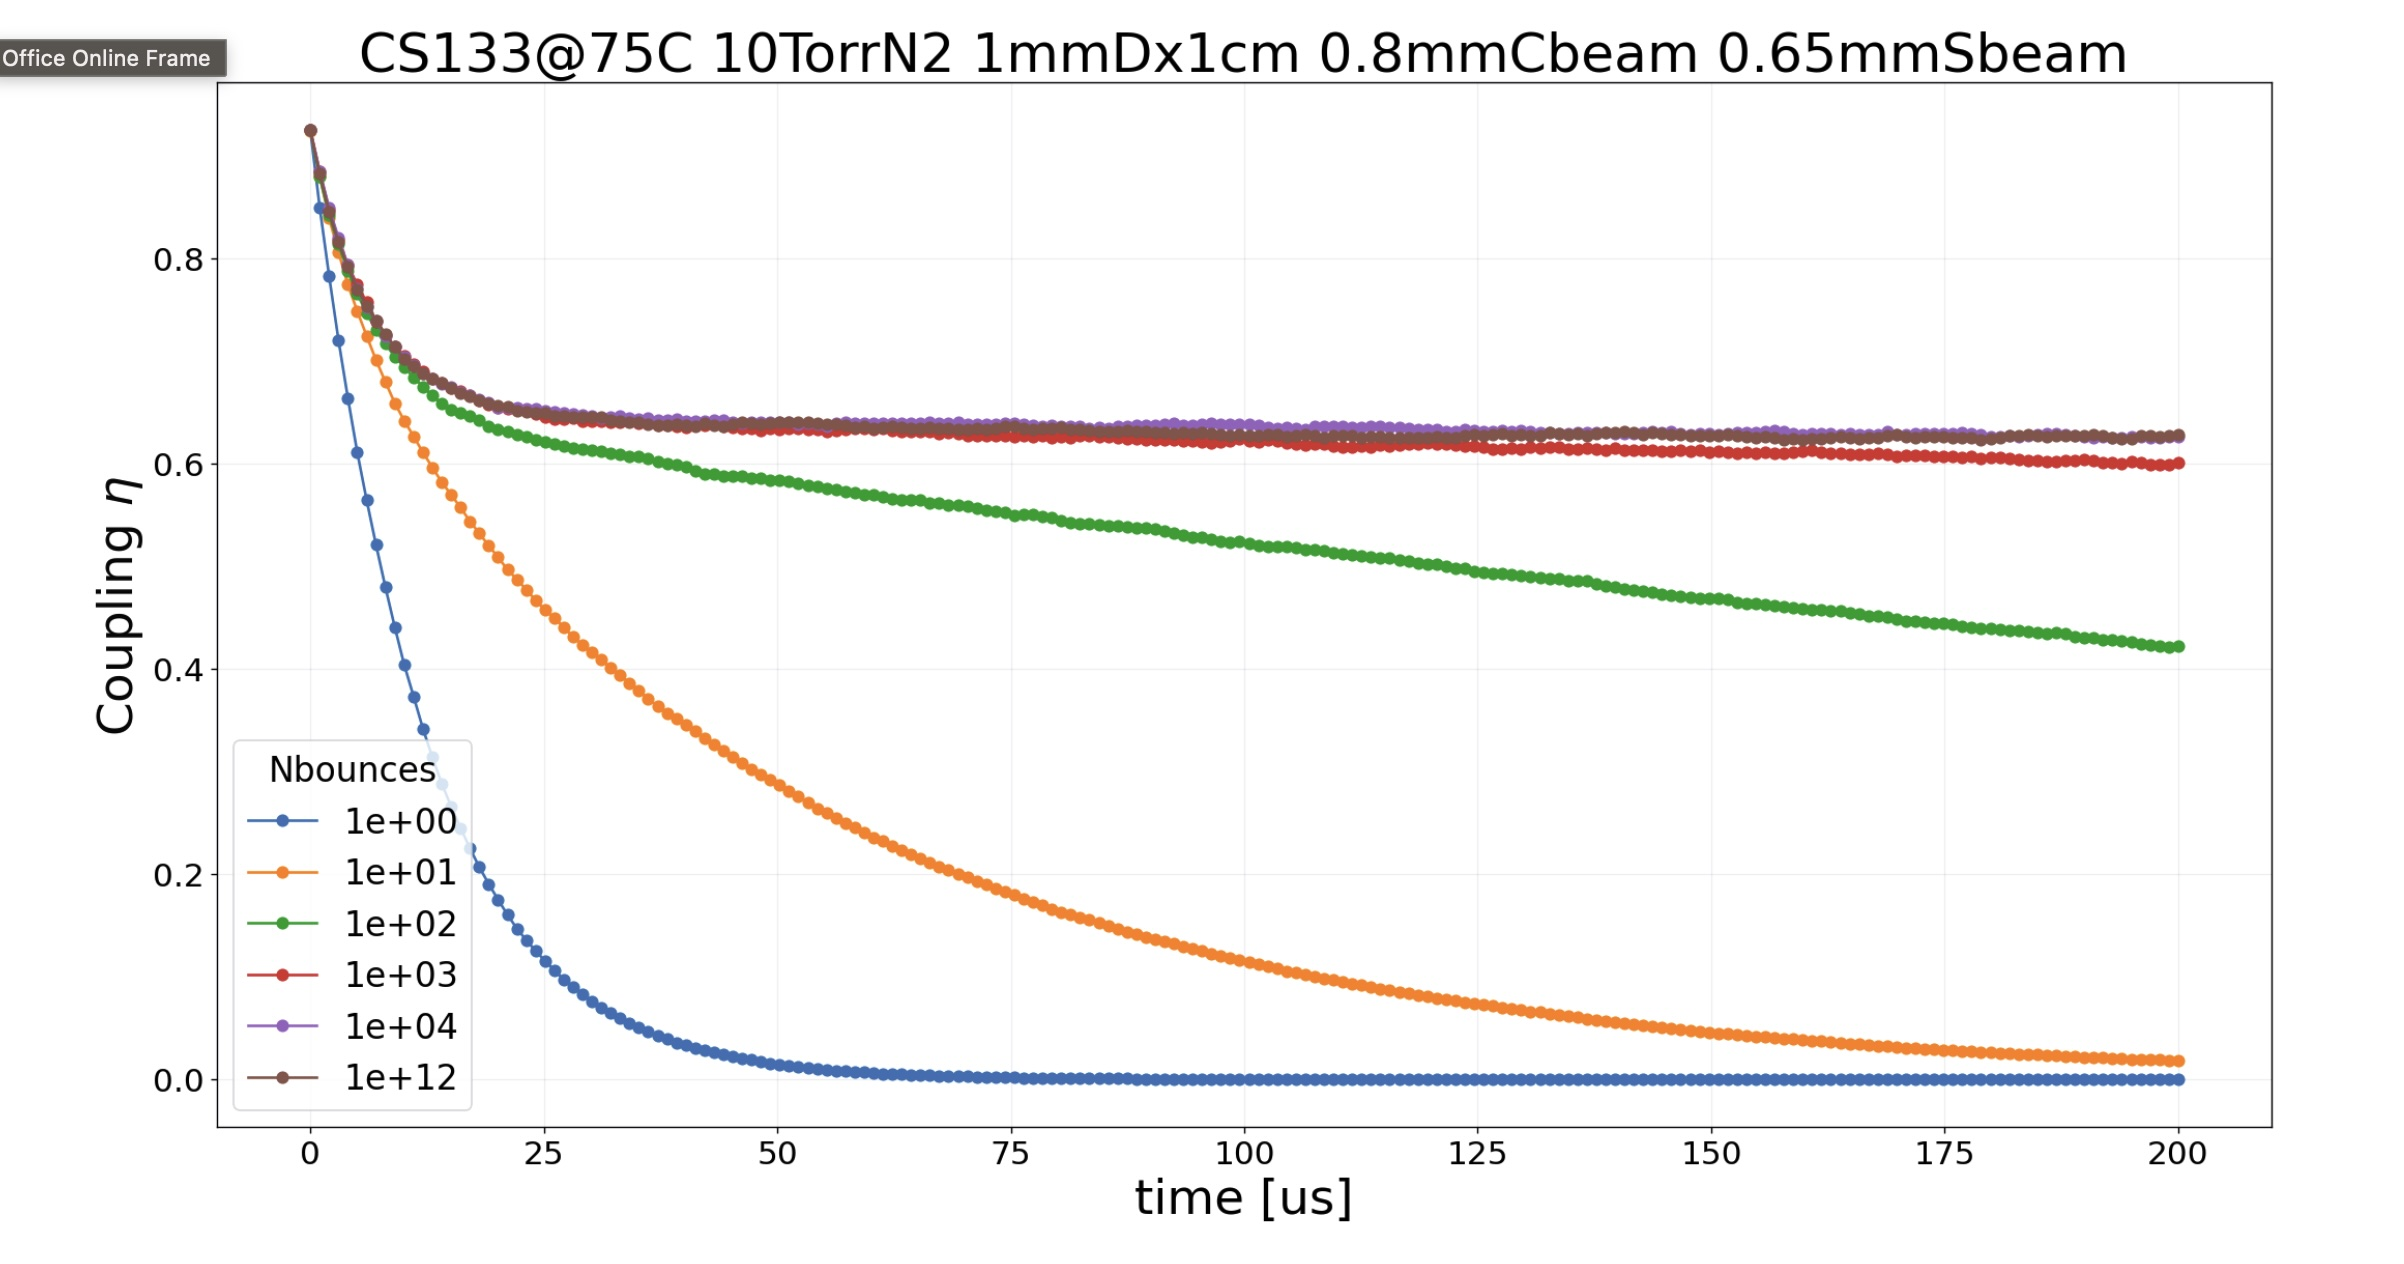
\includegraphics[width=0.72\textwidth]{Figures/coating_bounce_scan.jpeg}
\caption{Normalized fibre-coupled retrieval in the compact cell for different values of the mean coherence-preserving wall-collision number $N_{\mathrm{b}}$. The influence of the coating is strongest when wall-induced relaxation removes a substantial fraction of the atomic contributions from the coherent readout.}
\label{fig:coating_bounce_scan}
\end{figure}

The calculated coating dependence is shown in Fig.~\ref{fig:coating_bounce_scan}. At low $N_{\mathrm{b}}$, each encounter has an appreciable probability of destroying the $\ket{g}$--$\ket{s}$ coherence. The cylindrical wall then behaves as an absorbing boundary for the collective excitation, even though the simulated atom is mechanically reflected and remains inside the cell. Atoms that reach the wall are progressively removed from the amplitude sum, and the fibre-coupled retrieval decreases as the number of wall encounters grows.

Increasing $N_{\mathrm{b}}$ allows a larger fraction of the atoms to remain coherent after reaching the boundary. These atoms may subsequently diffuse back towards the optical axis and recover a non-negligible readout weight. The improvement is therefore most visible at storage times for which a significant part of the ensemble has already sampled the wall. The early-time behaviour can remain comparatively insensitive to the coating because many of the atoms have not yet reached the boundary.

The curves approach one another when $N_{\mathrm{b}}$ becomes sufficiently large. In this regime, the expected survival factor remains close to unity for the number of collisions accumulated during the simulated interval. Wall-induced depolarization is no longer the dominant source of retrieval loss. The remaining decay is then determined mainly by the spatial factor $u_{\mathrm{read}}(\mathbf{r}_j(t))$, motion away from the initially prepared spin-wave envelope, and any loss of collective phase alignment. Improving the coating beyond this point cannot recover atoms whose internal coherence survives but whose spatial contribution no longer matches the fibre mode.

A long tail or plateau at large $N_{\mathrm{b}}$ must consequently be interpreted with care. It does not demonstrate an indefinitely preserved memory. In a finite reflecting volume, atoms can leave the strongly weighted optical region and later return to it. When wall survival is high, these returning atoms can again contribute to the simulated coherent field. Such behaviour represents finite-volume diffusion and recurrence within the assumed boundary conditions. Additional experimental relaxation mechanisms, including residual magnetic gradients, spin-exchange collisions, coating inhomogeneity, and imperfect control-field coverage, would reduce this contribution in a physical cell~\cite{OP_Happer_1972,Apgteitiav_FinkelsteinEtAl_2023}.

For cell procurement, the coating should therefore be specified together with the intended operating temperature and alkali species. A quoted coating name alone is insufficient. The experimentally relevant information is the measured ground-state relaxation time or effective collision number after alkali exposure, under the temperature conditions expected during operation. The coating of the cylindrical wall, end caps, windows, and any stem connected to the vapour reservoir must also be considered, since atoms can sample each of these surfaces during long storage intervals.

\subsection{Cell Length Relative to the Spin-Wave Wavelength}
\label{sec:results_cell_length_spin_wave}

The effect of the cell length is governed by its relation to the axial spin-wave wavelength,
\begin{equation}
    \lambda_{\mathrm{SW},z}
    =
    \frac{2\pi}{|\Delta k_z|},
    \label{eq:results_axial_spin_wave_wavelength}
\end{equation}
where $\Delta k_z$ is the axial component of the spin-wave wave vector. The presence of several spin-wave periods within the cell does not by itself reduce retrieval, since the phase-matched readout addresses the corresponding collective mode. Dephasing arises when atomic motion changes the phase carried by each atom.

An axial displacement $\Delta z_j(t)=z_j(t)-z_j(0)$ produces the phase change
\begin{equation}
    \delta\phi_{j,z}(t)
    =
    \Delta k_z\Delta z_j(t)
    =
    \frac{2\pi\Delta z_j(t)}
         {\lambda_{\mathrm{SW},z}}.
    \label{eq:results_axial_motion_phase}
\end{equation}
Different atomic displacements therefore produce different phases, reducing the constructive interference in the coherent sum of Eq.~\eqref{eq:array_factor_general}.

In a short cell, the axial displacement is restricted to a range smaller than the spin-wave period. When $L\ll\lambda_{\mathrm{SW},z}$, the accessible phase spread remains smaller than $2\pi$, and the atomic contributions cannot become completely dephased. A residual coherent contribution consequently remains, producing the long-time plateau observed in the retrieval.

As the cell length becomes comparable to or larger than $\lambda_{\mathrm{SW},z}$, atoms can explore a broader part of the spin-wave phase pattern. Their phases then span a larger interval and cancel more completely. The reduction of the plateau with increasing $L$ therefore results from the larger range of motion-induced dephasing allowed by the cell geometry.
